% !TEX TS-program = XeLaTeX
% use the following command:
% all document files must be coded in UTF-8
\documentclass[english]{textolivre}
% build HTML with: make4ht -e build.lua -c textolivre.cfg -x -u article "fn-in,svg,pic-align"

\usepackage{longtable}
\usepackage{array}
%\usepackage{makecell}
\usepackage{adjustbox} 
\usepackage[table]{xcolor} 
\usepackage{graphicx}

\journalname{Texto Livre}
\thevolume{18}
%\thenumber{1} % old template
\theyear{2025}
\receiveddate{\DTMdisplaydate{2025}{3}{18}{-1}} % YYYY MM DD
\accepteddate{\DTMdisplaydate{2025}{5}{12}{-1}}
\publisheddate{\DTMdisplaydate{2025}{8}{27}{-1}}
\corrauthor{Cherish How}
\articledoi{10.1590/1983-3652.2025.58180}
%\articleid{NNNN} % if the article ID is not the last 5 numbers of its DOI, provide it using \articleid{} commmand 
% list of available sesscions in the journal: articles, dossier, reports, essays, reviews, interviews, editorial
\articlesessionname{articles}
\runningauthor{How, Abidin and  Zulkarnain} 
%\editorname{Leonardo Araújo} % old template
\sectioneditorname{Daniervelin Pereira}
\layouteditorname{Saula Cecília}

\title{``Your funny don’t land'': impoliteness and resonance in YouTube comments towards a stand-up comedian}
\othertitle{``Sua graça não cai bem'': impolidez e ressonância em comentários do YouTube em relação a uma comediante de \textit{stand-up}}
% if there is a third language title, add here:
%\othertitle{Artikelvorlage zur Einreichung beim Texto Livre Journal}

\author[1]{Cherish How~\orcid{0000-0002-9783-9173}\thanks{Email: \href{mailto:cherish@um.edu.my}{cherish@um.edu.my}}}
\author[1]{Najah Zainal Abidin~\orcid{0000-0001-8738-573X}\thanks{Email: \href{mailto:najah@um.edu.my}{najah@um.edu.my}}}
\author[1]{Nur Azwin Zulkarnain~\orcid{0009-0009-8976-4747}\thanks{Email: \href{mailto:azwin@um.edu.my}{azwin@um.edu.my}}}
\affil[1]{Universiti Malaya, Faculty of Languages and Linguistics, Department of English Language, Kuala Lumpur, Malaysia.}

\addbibresource{article.bib}
% use biber instead of bibtex
% $ biber article

% used to create dummy text for the template file
\definecolor{dark-gray}{gray}{0.35} % color used to display dummy texts
\usepackage{lipsum}
\SetLipsumParListSurrounders{\colorlet{oldcolor}{.}\color{dark-gray}}{\color{oldcolor}}

% used here only to provide the XeLaTeX and BibTeX logos
\usepackage{hologo}

% if you use multirows in a table, include the multirow package
\usepackage{multirow}

% provides sidewaysfigure environment
\usepackage{rotating}

% CUSTOM EPIGRAPH - BEGIN 
%%% https://tex.stackexchange.com/questions/193178/specific-epigraph-style
\usepackage{epigraph}
\renewcommand\textflush{flushright}
\makeatletter
\newlength\epitextskip
\pretocmd{\@epitext}{\em}{}{}
\apptocmd{\@epitext}{\em}{}{}
\patchcmd{\epigraph}{\@epitext{#1}\\}{\@epitext{#1}\\[\epitextskip]}{}{}
\makeatother
\setlength\epigraphrule{0pt}
\setlength\epitextskip{0.5ex}
\setlength\epigraphwidth{.7\textwidth}
% CUSTOM EPIGRAPH - END

% to use IPA symbols in unicode add
%\usepackage{fontspec}
%\newfontfamily\ipafont{CMU Serif}
%\newcommand{\ipa}[1]{{\ipafont #1}}
% and in the text you may use the \ipa{...} command passing the symbols in unicode

% LANGUAGE - BEGIN
% ARABIC
% for languages that use special fonts, you must provide the typeface that will be used
% \setotherlanguage{arabic}
% \newfontfamily\arabicfont[Script=Arabic]{Amiri}
% \newfontfamily\arabicfontsf[Script=Arabic]{Amiri}
% \newfontfamily\arabicfonttt[Script=Arabic]{Amiri}
%
% in the article, to add arabic text use: \textlang{arabic}{ ... }
%
% RUSSIAN
% for russian text we also need to define fonts with support for Cyrillic script
% \usepackage{fontspec}
% \setotherlanguage{russian}
% \newfontfamily\cyrillicfont{Times New Roman}
% \newfontfamily\cyrillicfontsf{Times New Roman}[Script=Cyrillic]
% \newfontfamily\cyrillicfonttt{Times New Roman}[Script=Cyrillic]
%
% in the text use \begin{russian} ... \end{russian}
% LANGUAGE - END

% EMOJIS - BEGIN
% to use emoticons in your manuscript
% https://stackoverflow.com/questions/190145/how-to-insert-emoticons-in-latex/57076064
% using font Symbola, which has full support
% the font may be downloaded at:
% https://dn-works.com/ufas/
% add to preamble:
% \newfontfamily\Symbola{Symbola}
% in the text use:
% {\Symbola }
% EMOJIS - END

% LABEL REFERENCE TO DESCRIPTIVE LIST - BEGIN
% reference itens in a descriptive list using their labels instead of numbers
% insert the code below in the preambule:
%\makeatletter
%\let\orgdescriptionlabel\descriptionlabel
%\renewcommand*{\descriptionlabel}[1]{%
%  \let\orglabel\label
%  \let\label\@gobble
%  \phantomsection
%  \edef\@currentlabel{#1\unskip}%
%  \let\label\orglabel
%  \orgdescriptionlabel{#1}%
%}
%\makeatother
%
% in your document, use as illustraded here:
%\begin{description}
%  \item[first\label{itm1}] this is only an example;
%  % ...  add more items
%\end{description}
% LABEL REFERENCE TO DESCRIPTIVE LIST - END


% add line numbers for submission
%\usepackage{lineno}
%\linenumbers

\hyphenation{pseu-do-nym-i-ty}

\begin{document}
\maketitle

\begin{polyabstract}
\begin{abstract}
The expressive freedom of social media often results in impoliteness. Interestingly, impoliteness can also appear creatively through the blending of original utterances with reused words or structures to create resonance. This study explores two research questions: (1) How do YouTube users express impoliteness toward an Asian American stand-up comedian’s performance, particularly regarding Malaysia and the MH370 tragedy? (2) Do these comments exhibit resonance, and if so, how does resonance function within their impoliteness strategies? Employing thematic analysis, this qualitative study categorizes 118 comments using Culpeper’s impoliteness triggers and Tantucci’s dialogic categorization model to identify resonance patterns. The findings reveal that users predominantly employed insults, unpalatable questions, pointed criticisms, sarcasm, and form-driven impoliteness triggers in response to the performance. Resonance was observed as users creatively echoed the comedian’s name, original joke lines, and nationality to insult and criticize her. Such strategies encouraged others to imitate or escalate face-threatening acts. Users also disguised offensive language by altering spellings to bypass content moderation, which enables the viral spread of impoliteness. Such acts not only foster impolite online behaviour but may also influence younger users to adopt similar means of avoiding repercussions. Thus, this study is crucial in understanding how impoliteness and resonance contribute to the spread of hostile discourse on social media. Its contribution lies in foregrounding the creative nature of impoliteness, particularly in multilingual contexts. By focusing on Malaysian English and Malay, this study enriches the field of pragmatics and socio-discursive dynamics of social media communication. 
\keywords{Impoliteness \sep Resonance \sep Creativity \sep Stand-up comedy \sep YouTube comments}
\end{abstract}

\begin{portuguese}
\begin{abstract}
A liberdade expressiva das mídias sociais frequentemente resulta em impolidez. Curiosamente, a impolidez também pode aparecer criativamente por meio da mistura de enunciados originais com palavras ou estruturas reutilizadas para criar ressonância. Este estudo explora duas questões de pesquisa: (1) Como os usuários do YouTube expressam impolidez em relação à performance de uma comediante de \textit{stand-up} asiático-americana, particularmente em relação à Malásia e à tragédia do voo MH370? (2) Esses comentários exibem ressonância e, em caso afirmativo, como a ressonância funciona em suas estratégias de impolidez? Empregando análise temática, este estudo qualitativo categoriza 118 comentários usando os gatilhos de impolidez de Culpeper e o modelo de categorização dialógica de Tantucci para identificar padrões de ressonância. As descobertas revelam que os usuários empregaram predominantemente insultos, perguntas desagradáveis, críticas diretas, sarcasmo e gatilhos de impolidez baseados em forma em resposta à performance. Observou-se ressonância quando usuários ecoaram criativamente o nome da comediante, suas piadas originais e sua nacionalidade para insultá-la e criticá-la. Tais estratégias incentivaram outros a imitar ou intensificar atos de ameaça à imagem. Usuários também disfarçaram linguagem ofensiva alterando a grafia para contornar a moderação de conteúdo, o que permite a disseminação viral da impolidez. Tais atos não apenas fomentam comportamentos online grosseiros, mas também podem influenciar usuários mais jovens a adotar meios semelhantes para evitar repercussões. Assim, este estudo é crucial para compreender como a impolidez e a ressonância contribuem para a disseminação de discurso hostil nas mídias sociais. Sua contribuição reside em destacar a natureza criativa da falta de educação, particularmente em contextos multilíngues. Ao se concentrar no inglês malaio e no malaio, este estudo enriquece o campo da pragmática e da dinâmica sociodiscursiva da comunicação nas mídias sociais.
\keywords{Impolidez \sep Ressonância \sep Criatividade \sep Comédia \textit{stand-up} \sep Comentários do YouTube}
\end{abstract}
\end{portuguese}
% if there is another abstract, insert it here using the same scheme
\end{polyabstract}

\section{Introduction}
Given that social media users often have the freedom to generate public outcry with impolite comments without facing consequences, impoliteness is commonly observed on social media. Social media platforms, such as YouTube, serve as spaces where hateful speech, violent comments, and messages are expressed to promote hatred \cite{matamorosfernandez2021, parvaresh2023}. This environment, coupled with the anonymity provided by social media, contributes to the escalation of impolite exchanges \cite{vladimirou2021}.

The effects of impoliteness can often be achieved through creativity \cite{culpeper2013}. While creativity plays a crucial role in entertaining impoliteness, it extends beyond mere entertainment \cite{culpeper2011}. There are two types of creativity: creativity as pattern re-forming and creativity as pattern forming. The former emphasises ``more overt, presentational uses of language", often involving idioms, metaphors, or puns \cite[p. 109]{carter2004}. For instance, the idiom ‘out of the frying pan into the fire’ can be reformed as ‘out of the frying pan into the deep freeze’ \cite[p. 95]{carter2004}. The latter, on the other hand, is ``less overt", and often involves ``parallelisms, echoes, and related matching of expressions" \cite[p. 109]{carter2004}. Pattern-forming in symmetrical situations includes repetition, escalation, and oppositions \cite{culpeper2011}. \textcite{tantucci2018} propose such a situation as a resonance. 

\textcite[p. 2461]{tantucci-wang2023} state that resonance occurs when ``a speaker draws on a prior utterance as a resource for producing a new one and selectively re-uses some of the words, structures, and other linguistic resources that were just uttered". Speakers occasionally generate impolite remarks by creatively recalibrating utterances that echo the forms and meanings of prior speakers’ expressions, using this approach as a means to offend their interlocutors. In the following example \cite[p. 301]{lein1978}, resonance is illustrated in the context of creative impoliteness:
\begin{description}
\item[James:] \emph{I sock you in} your nose.
\item[Art:] \emph{I sock you in} the mouth.
\item[James:] \emph{You gonna have a} black eye you keep on.
\item[Art:] \emph{You gonna have a} bloody nose, and a bloody mouth and knocks one of your teeth out. I’m gonna knock ‘em down your throat.
\end{description}

In this example, the second speaker re-uses linguistic items from the first speaker (``I sock you in ...", ``you gonna have a ..."). This phenomenon is also identified as pattern-forming impoliteness in symmetrical situations \cite[p. 243]{culpeper2011}.

In (im)politeness, recombinant creativity plays a prominent role as interlocutors need to understand the socio-normative nature of what might be considered impolite or offensive in different contexts \cite{tantucci2023}. In our study, for example, a user commented, ``Your funny don’t land", regarding Jocelyn Chia’s stand-up comedy performance posted on YouTube. This comment exemplifies resonance, as Chia’s original proposition in her joke was ``Some jokes don’t land". In this case, the user resonates with Chia’s structure at both syntactic and lexical levels. Syntactically, the user imitates the structure [DET joke[s] NEG X] but alters the determiner ‘some’ to ‘your’ and the noun ‘jokes’ to ‘funny’. Lexically, similar choices of lexical items were used: some $\rightarrow$ your; jokes $\rightarrow$ funny. This utterance is comprehensible only to those familiar with the content and context of the performance, as it serves as an insult to Chia. Individuals not involved in the context may not grasp the user’s comment. In terms of illocutionary force, Chia’s original utterance was an idiom, serving as a general statement that jokes are subjective to one’s view, while the user’s comment was targeted at criticising Chia’s performance. It can be speculated that the user commenting on the insult found Chia’s performance offensive. Consequently, ``an insult would ‘resonate’ leading to a reciprocal counter-insult" \cite[p. 10]{tantucci2018}.

Building on Culpeper and Tantucci’s \citeyear{culpeper2021} work, reciprocity in online interactions, particularly (im)politeness reciprocity and epistemic reciprocity, is shaped by both the immediate exchange (``here and now") and the record of previous interactions (``in the long term") \cite{oliveira2025}. Interactions on online platform take place asynchronously, where users may comment on a post or YouTube video weeks or even months later. In such digital spaces, the ``here and now" is not fixed by the original posting time but instead is reconstructed at the moment of user engagement. Each comment represents a user’s real-time reflection that is made ``immediate" through their personal opinion of the content or the resurfacing of public discourse around it \cite{oliveira2025}. This fluidity allows users to still participate in reciprocity using resonance by drawing from both the current and earlier interactions, which are readily accessible in comment threads. On the other hand, the ``in the long term" aspect of reciprocity refers to how social media users continue to draw on past interactions when formulating their comments \cite{oliveira2025}. In asynchronous platforms like YouTube, the comment thread acts as an archive, allowing users to access and respond to older posts. This longitudinal engagement strengthens the sense of affiliation and sustains impoliteness beyond the original timeframe of the video’s release \cite{oliveira2025}.

Thus far, studies on resonance in (im)politeness in digital interactions are still scarce. To address the gap, this paper delves into the exploration of resonance in the context of impoliteness. Specifically, the study aims to answer the following research questions:
\begin{itemize}
    \item How do YouTube users express impoliteness towards Jocelyn Chia’s stand-up comedy performance on June 7, 2023?
    \item Are there resonances in YouTube users’ comments? If so, how does resonance operationalise in their use of impoliteness strategies?
\end{itemize}

This study contributes to the field of pragmatics and socio-discursive dynamics by offering a novel analysis of impoliteness in a multilingual social media context. It demonstrates how users not only express impoliteness but also creatively manipulate it through resonance. By exploring how impolite language is replicated, modified, and made viral via resonance in user comments, this study expands the theoretical scope of impoliteness research to better understand the viral spread of hostile discourse online. Moreover, it highlights how Malaysian English and Malay languages shape impoliteness strategies and resonance patterns in social media discourse. 

\subsection{Impoliteness on social media and affiliations}
The tendency to commit impoliteness on social media is often associated with the anonymity, pseudonymity, and most importantly, affiliation. The cyber-psychological perception that perceives the sanctioning of harmful and insulting remarks is commonly elevated by such an ability of hiding behind the screen where manners are disregarded \cite{brown2018, kapoor2022, sinkeviciute2018, tagg2017, yun2020}. \textcite{andersson2021} reported that the consequential effect of impoliteness on social media such as YouTube can create a kind of social attachment among like-minded individuals to defend and uphold their stances and beliefs. This commonly results from the collective negative emotions that stem from taking offence, including triggering fear, aggression and motivation to represent their social groups.

According to \textcite{garces2013}, (dis)affiliation in/from a particular group is related to the construct of social identities. This construction process is greatly influenced by factors such as cultural background, social norms and experiences where they shape an individual’s sense of belonging to particular social groups that best represent them. Correspondingly, such an in-group affiliation practice causes taking offence to be done collectively as a group when their social identity is disrespected or harmed by their out-group counterpart \cite{alias2019, andersson2021}. From the shared offence taken, the communicative dynamic that exists among the homophily online community is largely provoked by their social norms and the specific audience that they intend to counter the offence \cite{tagg2017}.

Nonetheless, offences are not always taken negatively, especially in an online context. \textcite{boyd2014} revealed that aggressive and offensive comments on YouTube are often ignored. In fact, they are accepted as a positive reaction that could attract more users to participate in the discussion. Generally, rather than taking offence by the impoliteness caused by others who took offence at first, the addressee takes it as an opportunity to gain publicity.

\subsection{Creative impoliteness}
The ability to use language creatively can elevate one’s social status in digital interactions, provide emotional pleasure to observers, foster (dis)affiliative relationships, and align the speaker and non-targeted audiences against the target, reinforcing group membership dynamics \cite{andersson2023}. According to \textcite[p. 6]{culpeper2013}, ``impoliteness is often creative, and in fact achieves its effects through their creativity". He further explains that linguistic creativity lies in using words in unexpected and context-sensitive ways that encourage listeners or readers to infer meaning beyond the literal. In this regard, \textcite{culpeper2013} specifically referenced \textcite[p. 134]{carter2004}, who stated that ``the well-known truths expressed by proverbs are usually oblique and implicit rather than direct statements, they often have a metaphorical basis and their indirectness prompts interpretation and a ‘creative’ inferencing of meaning". 

This creative use of impoliteness is particularly evident in media discourse, such as TV shows. \textcite{kantara2010} highlights that sarcasm is a multifaceted tool that serves engaging and memorable functions. She further explains that in environments with unequal power dynamics, individuals may opt for sarcasm to align with their audience while navigating their position of authority and maintaining social harmony. Moreover, \textcite[p. 356]{culpeper1996} categorises sarcasm or mock politeness as instances where ``the FTA is performed with the use of politeness strategies that are obviously insincere, and thus remains surface realizations". This notion aligns with the findings of \textcite{bousfield2018}, who observed that people creatively modify offensive behaviour to influence others effectively. Interestingly, in environments where impoliteness is common and expected, creative impoliteness may be perceived as humorous rather than serious, highlighting the inventive nature of impolite expressions. This humour often arises from the unexpectedness or incongruity of the behaviour, a fundamental element of comedy \cite{raskin1985}.

Creative impoliteness can also be observed when well-known figures are mocked on social media. \textcite{vladimirou2018} term such act as ‘ludic impoliteness’ -- the playful yet collaborative form of mocking towards public figures on digital interaction. In their study on how Greek users mocked the English skills of political figures in Twitter/X discourse, \textcite{vladimirou2018} observed that the impoliteness was ludic as it was crafted through parody, mimicry, and humorous exaggeration. These acts of ridicule required inferential cooperation from the audience, who had to ``get the joke" by drawing on shared political and linguistic knowledge. Thus, creative impoliteness here becomes a kind of cultural performance, both playful and critical. This interplay between creativity and impoliteness on public figures is further explored in Oliveira and Miranda’s \citeyear{oliveira2024} study of Twitter/X responses to the 2022 Brazilian presidential debate. They introduce the concept of impoliteness metadiscourse, where users, often uninvolved bystanders, evaluate and reciprocate politicians’ verbal behaviour through stylised sarcasm, hashtags, and negative assertions. These responses were not random or purely emotional; rather, they were deliberate and creatively constructed, drawing on shared cultural knowledge and norms. The creativity lies in how users transformed impolite behaviour into socially resonant commentary, using irony, parody, and intertextuality to express judgement and forge alignment. In both studies, creative impoliteness emerges not just as a form of entertainment, but as a socially meaningful act that requires audiences to infer deeper meaning and participate in collective evaluations of morality, particularly towards public figures.

\subsection{The concept of resonance}
\textcite[p. 372]{dubois2014} defined resonance as the ``catalytic activation of affinities across utterances". In other words, resonance takes place when interlocutors creatively combine the original utterance of the previous speaker with a new one that is formally and phonetically similar \cite{tantucci2021}. This involves interlocutors repeating a linguistic item or creatively varying the syntactic structure from the utterance of a prior speaker \cite{tantucci2022b}.

The concept of resonance is driven by the Principle of (Im)politeness Reciprocity (PIR) and the Principle of Epistemic Reciprocity (PER). \textcite{culpeper2021} introduce the PIR, which frames (im)politeness as a social mechanism of reciprocity. For instance, insults often trigger similar responses, likely motivated by a need to avoid seeming weak or submissive by staying silent. Building on this, \textcite{tantucci2022} propose the PER, which governs the reciprocal obligations individuals feel when engaging in knowledge exchange. This is further elaborated through two maxims: (1) the Engagement Maxim ($E$), which emphasizes active interest in an interlocutor’s contributions, and (2) the Knowledge Exchange Maxim ($Ke$), which pertains to mutual investment in shared learning or understanding.

Resonance can be employed by social media users to creatively express impoliteness, such as sarcasms or insults, in order to make their comments stand out. Such comments not only serve to retaliate, but also fulfil the Engagement Maxim as it enhances engagement by attracting attention and resonating with other users. \textcite[p. 247]{tantucci2023} states that speakers often imitate and reformulate the utterances and behaviours of the prior speakers in a creative manner to ``produce a new meaning or perform a new action". In this case, the speaker does not just merely imitate what the previous speaker said, but instead adjusts and creates a new meaning or response \cite{tantucci2023}. This process is known as recombinant creativity. Recombinant creativity reinforces dynamic resonance. 

In an example by \textcite[p. 10]{tantucci2018}, resonance plays a role in terms of structure and influences the illocutionary forces.
\begin{description}
\item[A:] Alright Martin. \emph{I’ll see you later}.
\item[B:] \emph{I’ll see you later anyway}. I’ll.
\item[A:] Okay. Yeah.
\end{description}


In this example, resonance can be seen in B’s response when he repeats A’s utterance ‘I’ll see you later’ and further adds the pragmatic marker ‘anyway’, which changes the illocutionary forces from greeting to commissive. \textcite{tantucci2023} further added that such creative alteration of the original proposition serves as an ‘on record’ engagement with the speaker. This shows that language use is not just fixed phrases, but is inherently flexible and adaptive. Speakers can re-use and modify elements of what others say, whether in structure, meaning, or intent, to form new expressions that align morphosyntactically, semantically, and pragmatically \cite{dubois2014}. Similarly, interlocutors can express impoliteness creatively by re-using and modifying the words of the target. Creative resonance is a core aspect of interactional engagement, as it explicitly signals alignment with another interlocutor’s utterance \cite{tantucci2024}. While such resonance often acts as a positive face booster, it can also be used to reinforce face-threatening acts.

\section{Methodology}
This study exclusively focuses on a Singaporean raised American comedian, Jocelyn Chia, specifically the YouTube comments of disapproval from social media users regarding her comedy performance on June 7, 2023. The YouTube video featured Jocelyn Chia making jokes about Malaysia removing Singapore from the country and the tragedy of MH370. Her jokes became controversial and sparked a public outcry. The full version of her video performance was removed from social media, leaving only this short, edited video clip featuring her Malaysia-Singapore and MH370 jokes available on YouTube. This video was one minute and nineteen seconds long. Despite its short length, there were 866 comments on the YouTube video at the time of data collection, including replies to other commenters, which had a total of 15,619 views. This data was manually collected nine months after the clip originally aired on June 18, 2023, uploaded by the comedian. 

The comments were mainly written in English, with some in Malay and Chinese. There are 155 comments that directly responded to the video. Out of these comments, a total of 118 comments that expressed disapproval and contained impoliteness on Jocelyn Chia’s stand-up comedy performance in the aforementioned video were analysed. Replies to other commenters and comments with only emoticons were excluded. Our focus was on exploring the way social media users respond to Chia’s performance rather than other commenters’ views.

Following Henrich and Holmes’ \citeyear{henrich2013} criteria for comment inclusion, we only included comments containing impolite instances, as the aim of this study is to examine impoliteness in the YouTube comments of the selected video. Comments targeting other commenters were excluded, as this study focuses solely on comments directed at the stand-up comedian. For the purpose of reliability and consistency, we cross-checked each other’s categorisation of impoliteness strategies and identification of resonance in impoliteness. In cases of intercoder differences, we revised our coding through discussion. 

This study not only focuses on Malaysian users but also includes non-Malaysian users who disapproved of Chia’s performance. Given that we were unable to distinguish the nationality of the commenters due to anonymity and only a handful of them mentioned their nationality in their comments, users’ nationalities could not be identified and confirmed. Thus, we did not specify the commenters’ nationality in our analysis. Nevertheless, the focus of this study is on how the users linguistically express impoliteness with resonance, which can be analysed regardless of explicit user identity. For confidentiality purposes, all usernames and profile pictures in the comments were pseudonyms.

The data were examined for instances of epistemic (mis)matching by analyzing how users oriented to Chia’s comedy performance and contested epistemic authority in their comments. Particular attention was given to comments that reclaimed epistemic rights through impoliteness triggers and resonance, indicating perceived mismatches between Chia’s epistemic efforts and the audience's expectations.

To answer the first research question, Culpeper’s \citeyear{culpeper2011} conventionalised and non-conventionalised impoliteness formulae were adopted to scrutinise how social media users expressed their disparagement for Chia’s performance. In this instance, we also explored the data using thematic analysis as the approach.

\begin{itemize}
\item Conventionalised impoliteness formulae
    \begin{itemize}
    \item Insults
    \item Pointed criticisms or complaints
    \item Unpalatable questions or presuppositions
    \item Condescension
    \item Message enforcers
    \item Dismissals
    \item Silencers
    \item Threats
    \item Negative expressions
     \end{itemize}
\item Non-conventionalised impoliteness formulae
    \begin{itemize}
    \item Form-driven
    \item Convention-driven (internal and external)
    \item Context-driven (unmarked behaviour and absence of politeness)
     \end{itemize}
\end{itemize}

To answer the second research question, one of the conditions of Tantucci’s \citeyear{tantucci2023} dialogic categorisation model (DCM) was employed to identify resonance, which is as follows: ``There must be at least one lexical unit -- including interjections or pragmatic markers -- being repeated from interlocutor A to B" \cite[p. 363]{tantucci2023}. This condition guided our analysis of resonance in the context of impoliteness.

\section{Analysis of impoliteness triggers in the comments}
The occurrences of conventionalised impoliteness triggers instances are shown in Table \ref{tab-1}, where insults emerged as the most prominent impoliteness trigger, with a total of 30\% observed. Within this category, personalised negative references, personalised third-person negative references, personalised negative vocatives, and personalised negative assertions were notably prevalent. Following insults, unpalatable questions/presuppositions (12\%) and pointed criticism/complaints (10\%) were also significant impoliteness triggers. Other impoliteness triggers which showed minimal occurrence were negative expressive (8\%), condescension (4\%), threats (3\%), message enforcers (2\%), and silencers (1\%). However, dismissals showed no occurrence (\Cref{fig-1}).

%--- CÓDIGO DA TABELA 1 ---%
\begin{table}[h!]
\centering
\begin{threeparttable}
\caption{Conventionalised impoliteness triggers percentages.}\label{tab-1}
\begin{tabular}{lr}
\toprule
Conventionalised impoliteness triggers & \multicolumn{1}{c}{Percentages} \\
\midrule
Insults & 30\% \\
\quad a. Personalised negative reference & 12\% \\
\quad b. Personalised third-person negative reference & 8\% \\
\quad c. Personalised negative vocatives & 6\% \\
\quad d. Personalised negative assertion & 4\% \\
Unpalatable questions and/or Presuppositions & 12\% \\
\quad a. Unpalatable questions & 8\% \\
\quad b. Presuppositions & 4\% \\
Pointed criticism / complaints & 10\% \\
Negative expressive (curses / ill-wishes) & 8\% \\
Condescension & 4\% \\
Threats & 3\% \\
Message enforcers & 2\% \\
Silencers & 1\% \\
Dismissals & 0\% \\
[0.5em]
Total & 70\% \\
\bottomrule
\end{tabular}
\source{Own elaboration.}
\end{threeparttable}
\end{table}

%--- CÓDIGO DA FIGURA 1 ---%
\begin{figure}[h!]
    \centering
    \begin{minipage}{0.85\linewidth}
    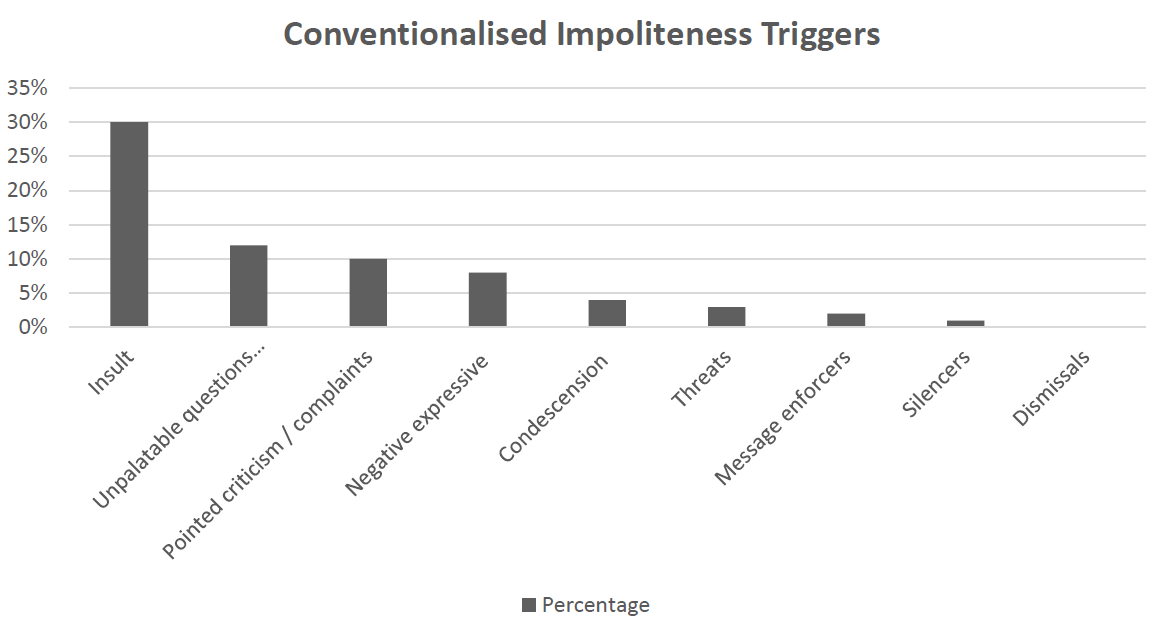
\includegraphics[width=\linewidth]{imagens/figura1.png}
    \caption{Conventionalised impoliteness triggers.}\label{fig-1}
    \source{Own elaboration.}
    \end{minipage}
\end{figure}

Table \ref{tab-2} illustrates that convention-driven (20\%) exhibits the highest percentage among the non-conventionalised impoliteness triggers, with external convention-driven implicational impoliteness (sarcasm) and diachronic internal convention-driven implicational impoliteness each noted in 16\% and 4\% of occurrences respectively. Additionally, form-driven implicational impoliteness (resonance) displays moderate occurrences (10\%). Conversely, synchronic internal convention-driven implicational impoliteness, context-driven implicational impoliteness (unmarked behaviour), and context-driven implicational impoliteness (absence of politeness) were not observed in the study (\Cref{fig-2}).
\newpage

%--- CÓDIGO DA TABELA 2 ---%
\begin{table}[h!]
\centering
\begin{threeparttable}
\caption{Non-conventionalised impoliteness triggers percentages.}\label{tab-2}
\begin{tabular}{lc}
\toprule
Non-conventionalised impoliteness triggers & Percentages \\
\midrule
Convention-driven & 20\% \\
\quad a. External convention-driven implicational impoliteness (sarcasm) & 16\% \\
\quad b. Diachronic internal convention-driven implicational impoliteness & 4\% \\
\quad c. Synchronic internal convention-driven implicational impoliteness & 0\% \\
Form-driven: implicational impoliteness & 10\% \\
\quad a. Resonance (mimicry) & 10\% \\
Context-driven & 0\% \\
\quad a. Context-driven implicational impoliteness (unmarked behaviour) & 0\% \\
\quad b. Context-driven implicational impoliteness (absence of politeness) & 0\% \\
[0.5em]
Total & 30\% \\
\bottomrule
\end{tabular}
\source{Own elaboration.}
\end{threeparttable}
\end{table}

%--- CÓDIGO DA FIGURA 2 ---%
\begin{figure}[h!]
    \centering
    \begin{minipage}{0.85\linewidth}
    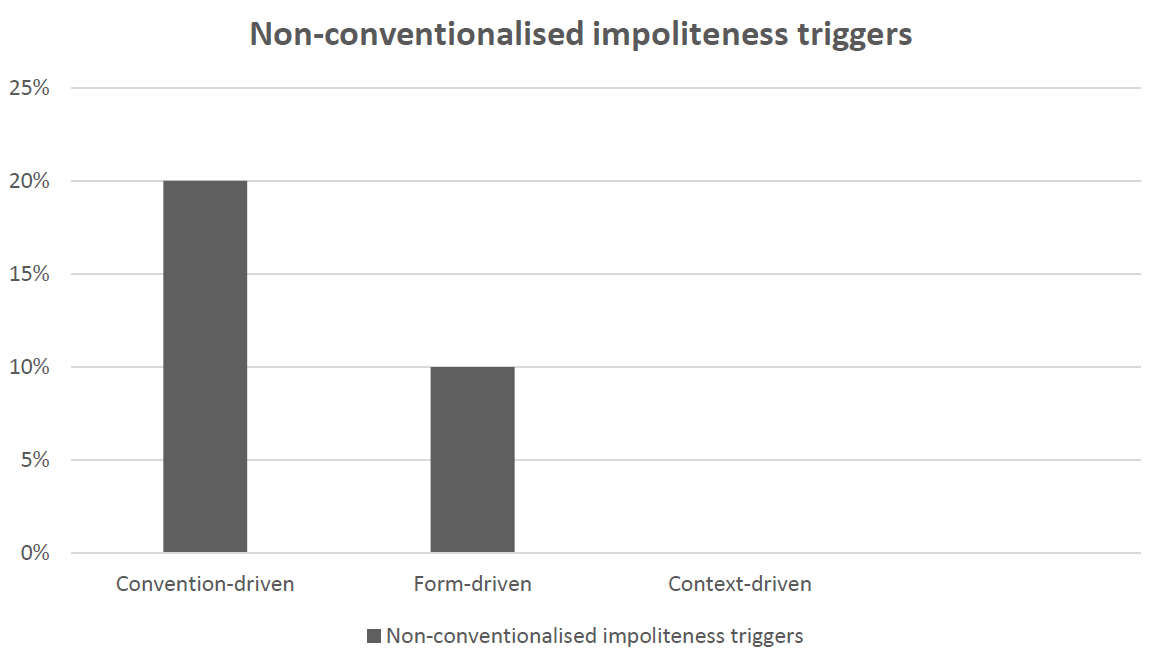
\includegraphics[width=\linewidth]{imagens/figura2.png}
    \caption{Non-conventionalised impoliteness triggers.}\label{fig-2}
    \source{Own elaboration.}
    \end{minipage}
\end{figure}

Based on our analysis, we discovered various impoliteness triggers employed by social media users to attack the comedian’s face. In Table \ref{tab-3}, we provide some examples of both conventionalised and non-conventionalised impoliteness triggers found in the data.

%%--- CÓDIGO DA TABELA 3 ---%
\begin{longtable}{p{6.5cm} p{7.5cm}}
\caption{Examples of (non)conventionalised impoliteness triggers in the data.}\label{tab-3}\\
\toprule
{(Non)conventionalised impoliteness triggers} & Examples \\
\midrule
Insult & \\
\quad \hspace{1em} a. Personalised negative vocatives & aunty kiasu not funny at all la aunty..aunty or anak dara tua \\
\arrayrulecolor{gray!70}\cmidrule(l{2em}){1-2}
\quad \hspace{1em} b. Personalised negative assertion & Look AT THOSE NEGATIVE FEEDBACKS U RECEIVE! \\ 
\arrayrulecolor{gray!35}\cline{2-2}
 & you must have some really thick skin to still ``laugh" at SG and M’sia for being sensitive. \\ 
\arrayrulecolor{gray!70}\cmidrule(l{2em}){1-2}
\quad \hspace{1em} c. Personalised negative reference & you brain under my feet \\
\arrayrulecolor{gray!70}\cmidrule(l{2em}){1-2}
\quad \hspace{1em} d. Personalised third person negative refe\-rence & she's a bitch \\
\arrayrulecolor{gray!35}\cline{2-2}
 & WITHOUT MALAYSIA SHE NOTHING \\
\arrayrulecolor{gray!35}\cline{2-2}
\arrayrulecolor{gray!70}\hline
Pointed criticism or complaint & your joke is not well received here (M’sia \& S’pre) to the majority of the people. it fell so flat (lacking skills to pull off that risky bit) \\ 
\arrayrulecolor{gray!35}\cline{2-2}
 & I really don’t like the way her joke! Very insulting \\ 
\arrayrulecolor{gray!35}\cline{2-2}
 & This is about how inappropriate the rude and immature behavior of Jocelyn Chia \\
\arrayrulecolor{gray!70}\hline
Unpalatable questions and/or presuppositions & \\
\quad \hspace{1em} a. Unpalatable questions & As if you care, right? \\ 
\arrayrulecolor{gray!35}\cline{2-2}
 & Why in hiding?? Scared of being slapped???! \\ 
\arrayrulecolor{gray!70}\cmidrule(l{2em}){1-2}
\quad \hspace{1em} b. Presuppositions & even her country disowned her..she has some serious mental issue..her ex bf must have been a malaysian.. \\
\arrayrulecolor{gray!70}\hline
Negative expressive (curses / ill-wishes) & I pray that the loved ones of this woman will also be involved in a plane crash accident. Let's see where her EGO will be if that happens \\ 
\arrayrulecolor{gray!35}\cline{2-2}
 & Still not die ah this bij? \\
\arrayrulecolor{gray!35}\cline{2-2}
\arrayrulecolor{gray!70}\hline
Condescension & did you tell them about how Shxtgaporean come over Malaysia just to pump the petrol like Sin don’t have petrol station? Yikesssssssssss \\
\arrayrulecolor{gray!70}\hline
Threats & don’t mess around with SEA netizens \\
\arrayrulecolor{gray!70}\hline
Message enforcers & we grew up in a different environment, you understand? \\ 
\arrayrulecolor{gray!35}\cline{2-2}
 & JOCELYN, YOU OWE FROM ALL THE MALAYSIAN AN APPOLOGY!!!! \\
\arrayrulecolor{gray!35}\cline{2-2}
\arrayrulecolor{gray!70}\hline
Silencers & Diam la ahsoh tua! (Shut up old lady!) \\
\arrayrulecolor{gray!70}\hline
External convention-driven implicational impoliteness (sarcasm) & You make this job look really easy. All you need to do to be “successful” is to insult others? \\ 
\arrayrulecolor{gray!35}\cline{2-2}
 & only 50 people were killed in this tragedy, very little and it’s so funny, isn’t it? \\
\arrayrulecolor{gray!35}\cline{2-2}
\arrayrulecolor{gray!70}\hline
Diachronic internal convention-driven implicational impoliteness & Why all people bully her, she has innocent face..seem like bossku najis, bruh \\
\arrayrulecolor{gray!70}\hline
Form-driven implicational impoliteness (resonance/mimicry) & Porcelain Chia, Goblyn Chia, Chiakimak \\ 
\arrayrulecolor{gray!35}\cline{2-2}
 & Shxtgaporean \\ 
\arrayrulecolor{gray!35}\cline{2-2}
 & your funny don’t land \\ 
\arrayrulecolor{gray!35}\cline{2-2}
 & Some joke dont lane but you brain under my feet \\
\arrayrulecolor{black}
\bottomrule
\source{Own elaboration.}
\end{longtable}

In the following subsections, we provide examples of analyses of impoliteness and resonance.

\subsection{Insults}
One of the triggers for impoliteness identified in the study involves insults containing personalised negative vocatives, assertions, and references, both in the second and third person \cite{culpeper2011}.

%--- CÓDIGO DO EXEMPLO 1 ---%
\begin{figure}[h!]
    \centering
    \begin{minipage}{0.70\linewidth}
    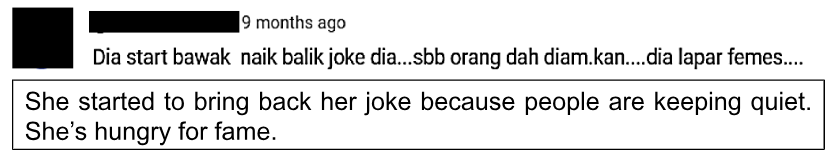
\includegraphics[width=\linewidth]{imagens/figura3-junto.png}
    \caption{Example 1.}
    \label{example-1}
    \source{\cite{jocelyn2023malaysian}.}
    \end{minipage}
\end{figure}

The comment \textit{``dia lapar femes…"} (she’s hungry for fame) in Example 1 (\Cref{example-1}) exemplifies the pattern of insult. This aligns with what \textcite{bousfield2007} mentioned -- that a trigger must have occurred for an impolite utterance to be spoken. The context triggering these insults was the comedic act performed by Jocelyn Chia regarding the disappearance of MH370. In response, insults, defined as ``a remark that puts someone down, or ascribes a negative characteristic to them" \cite[p. 20]{hay2002}, were reciprocated due to the failed attempt at humour by Chia. The intention was to offend the target \cite{dynel2019, hay2002}, which in this case, was Chia. The directness and intensity of the insult clearly portrayed a strong speaker commitment to the negative evaluation. This can be regarded as an attempt to assert social and epistemic authority over the appropriateness of Chia’s joke. 

Furthermore, the repeated use of personalized negative associations toward Chia also suggests an assumption of shared disapproval of the joke, thereby reinforcing a common group identity opposed to the act in its entirety. Similar to the impoliteness used in \textcite{han2021}, it was noted that impoliteness is viewed as a rhetorical or discursive strategy in the literature.

Han’s \citeyear{han2021} study discovered that blunt slogans may have been intentionally crafted to optimise their effectiveness to fulfil the prevention function during the coronavirus pandemic. In both cases, impoliteness serves a communicative purpose. Just as the response to the blunt slogans involved refuting criticism and remarking on the effectiveness of the approach \cite{han2021}, the impolite comments in the study were reciprocated due to a failed attempt at humour. Both contexts highlight the intention behind impoliteness and the reactions it elicits.

\subsection{Unpalatable questions}
Unpalatable questions were identified in the data. These questions attack the addressee’s face and they do not require responses.

%--- CÓDIGO DO EXEMPLO 2 ---%
\begin{figure}[h!]
    \centering
    \begin{minipage}{0.7\linewidth}
    
\includegraphics[width=\linewidth]{imagens/figura4.png}
    \caption{Example 2.}
    \label{example-2}
    \source{\cite{jocelyn2023malaysian}.}
    \end{minipage}
\end{figure}

Example 2 (\Cref{example-2}) illustrates users mocking the negative reviews Chia received for her comedy performance. The user questions Chia’s decision to omit the final part of her performance in the uploaded YouTube video. Obviously, this question is not meant to elicit a response from Chia. The unpalatable question “Ms [Miss] getting bad yelp review?”, which was sarcasm, served to prompt Chia to reflect on the repercussions of her actions. These indicate that her performance was poorly received by the public.

In relation to its acceptability by other commenters, such a question functions as a rhetorical device, where the user implicitly assumes a shared negative and critical stance embedded in the question. This adds a greater creativity and impact on the comment \cite{andersson2023}, thereby strengthening the attack on Chia’s face.

\subsection{Presuppositions}
Presupposition refers to one’s assumption that their utterance is true, which can serve to manipulate others and establish certain ideologies when expressing one’s assumption or opinion \cite{chen2019}. The following comment (\Cref{example-3}) illustrate how social media users who are against Jocelyn Chia’s stand-up comedy performance employed presuppositions to attack her face.

%--- CÓDIGO DO EXEMPLO 3 ---%
\begin{figure}[h!]
    \centering
    \begin{minipage}{0.70\linewidth}
    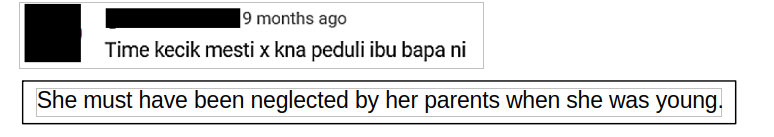
\includegraphics[width=\linewidth]{imagens/Fig5.png}
    \caption{Example 3.}
    \label{example-3}
    \source{\cite{jocelyn2023malaysian}.}
    \end{minipage}
\end{figure}

The users presuppose that the comedian’s controversial performance was influenced by the notion that she was neglected by her parents (\textit{``mesti x kna peduli ibu bapa ni"}). This suggests a shift in focus to her parents, who are blamed for her controversial stand-up comedy performance. Such presuppositions also reflect the ‘subjective assumptions’ \cite{chen2019} of the commenters towards Chia. Furthermore, presuppositions are evident in the use of the modal verb \textit{‘mesti’} (must), which serves to reinforce the user’s assumptions that her decision to perform controversial comedy is largely influenced by neglect from her parents. This suggests that the interactional impact of presuppositions depends on the extent to which the user believes in a common ideological framework among the commenters, shaped by their shared linguistic and cultural background. Besides, studies have shown that there is a direct correlation between the familial bond between Asian parents and children and how it facilitates the development of one’s way of communicating and learning \cite{awde2009}. Nonetheless, given that this statement was made without evidence, it can be classified as a presupposition since it is solely the assumption of the user, which is impolite because it consists of negative assumptions about Chia.

\subsection{Pointed criticism or complaint}
Impoliteness in view of pointed criticism or complaint is related with the expression of disapproval of the way of others \cite{kapoor2022}.

%--- CÓDIGO DO EXEMPLO 4 ---%
\begin{figure}[h!]
    \centering
    \begin{minipage}{0.80\linewidth}
    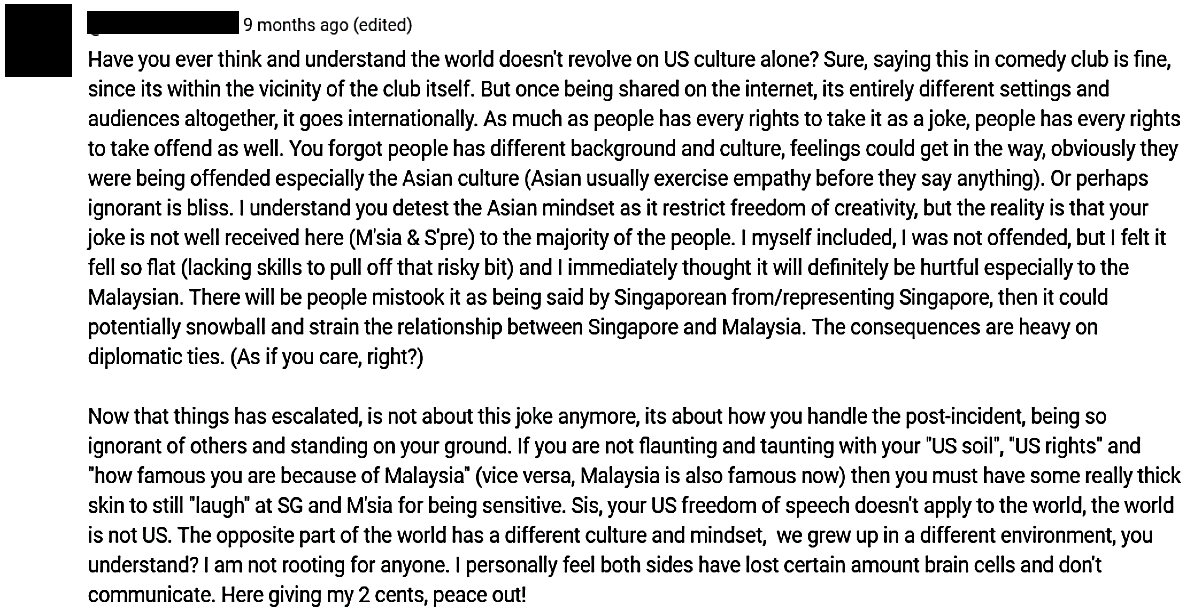
\includegraphics[width=\linewidth]{imagens/figura6.png}
    \caption{Example 4.}
    \label{example-4}
    \source{\cite{jocelyn2023malaysian}.}
    \end{minipage}
\end{figure}

Based on this example (\Cref{example-4}), the user shows his/her disapproval of the joke made by the comedian by highlighting that Malaysians taking offence is considered reasonable due to the contradictory background and cultural practices. On a contextual level, it is clear that the user relates Chia’s mockery with her lack of attentiveness towards the Asian culture that is said to insist on empathy above all.

In accordance with \textcite{spencer-oatey2016}, certain elements of (im)politeness may be fundamental within a language or cultural aspect of a community but may not hold the same importance or relevance within another. This suggests Chia’s obliviousness to the cultural consideration of the audience that might feel emotionally attacked insofar by the joke. The user then proceeds with a critical remark on the joke in which it was described as ``fell so flat" and that the comedian lacks skills in upholding an antagonistic behaviour in her joke. Such a direct manner of criticising is deemed to intentionally cause offence to Chia to imply her inadequacy in carrying out her role as a comedian. The confident tone in the user's evaluative stance, embedded in the comment, reflects a known cultural standard used to validate their criticism. For this reason, the pointed criticism reflected in this instance is not spontaneous at all. Instead, the presence of common-sense reasoning proffered by the user demonstrates the very reason for the expression of hate by social media users, which suggests the inaccurate representation by \textcite{brown2018} on the tendency for spontaneous forms of hate speech in online settings.

\subsection{External convention-driven implicational impoliteness: Sarcasm}
Another prevailing strategy that users tend to be inclined in expressing impoliteness towards Chia’s comedy performance is the external convention-driven implicational impoliteness where it signifies mock politeness/sarcasm. According to \textcite{culpeper2005, culpeper2011}, this strategy is not explicitly expressed as a form of impoliteness, as the speaker would opt for a politeness strategy instead that is deliberately made insincere.

%--- CÓDIGO DO EXEMPLO 5 ---%
\begin{figure}[h!]
    \centering
    \begin{minipage}{0.90\linewidth}
    
\includegraphics[width=\linewidth]{imagens/figura7.png}
    \caption{Example 5.}
    \label{example-5}
    \source{\cite{jocelyn2023malaysian}.}
    \end{minipage}
\end{figure}

In Example 5 (\Cref{example-5}), the semantic interpretation of the user’s comment simply delineates the user’s offering of suggestions on different topics for Chia’s future skit. However, the topics suggested are all of similar conception, that is, based on tragedies occurred in different countries. With the intent of bringing up controversial issues that might spark polarised ideologies \cite{tagg2017}, the user’s strategy to cause offence to Chia is seen as an act of implied disparagement in which the comedian’s lack of empathy towards agonising tragedies is inferred. In fact, such a strategy of impoliteness is blatantly expressed with a challenge where the user condemns Chia’s ability to make jokes out of the loss of others. It might be the case that the sense of provocation in this instance is influenced by the user’s manner of vocalising his/her anger towards the comedian. Besides, the attribution of ``the funniest stand-up comedian in the world" to Chia further suggests the sarcastic impression of the statement -- still advertising her indifference to public perceptions and feelings, as the user concludes his/her comment. This subtle form of impoliteness and indirectness relies heavily on shared knowledge and cultural frames of reference for other commenters to interpret it as offensive rather than complimentary. As such, the user positions themselves as speaking on behalf of others who have taken offense at her. 

\section{Analysis of the use of resonance in impoliteness}
With regard to creatively constructing impoliteness, the following types of resonance were identified in the users’ comments: resonance on Chia’s names, Singaporean nationality, Chia’s original joke lines ``Some jokes don’t land" and ``Aww!!! Booo!!!". Resonance on word, phrase, and sentence or utterance levels were constructed by social media users to creatively insult Chia’s names, Singaporean nationality, and her original joke lines. They are also considered form-driven implicational impoliteness (\Cref{fig-3}).

%--- CÓDIGO DA FIGURA 3 ---%
\begin{figure}[h!]
    \centering
    \begin{minipage}{0.85\linewidth}
    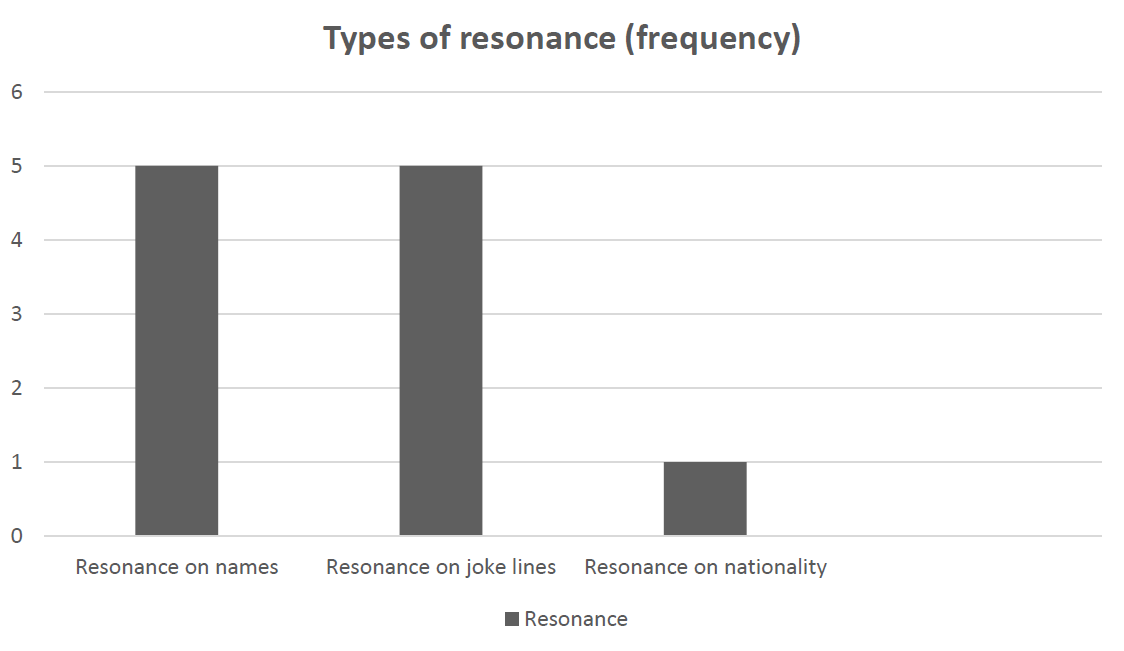
\includegraphics[width=\linewidth]{imagens/figura8.png}
    \caption{Types of resonance.}\label{fig-3}
    \source{Own elaboration.}
    \end{minipage}
\end{figure}

In the context of this study, the users’ comments on Chia’s YouTube video demonstrate a level of creativity with the use of resonance, such as mock spellings and parodic references. Although these comments are primarily aimed at attacking the comedian, they also function as a means of fostering social engagement and reinforcing participatory alignment among users \cite{xie2018}. This observation aligns with \textcite{oliveira2025}, who highlights the creative potential of digital interactions.

\subsection{Resonance on names}
Resonance on Chia’s first name and last name was found in the data where users creatively altered her original name ‘Jocelyn Chia’ to insult her.

%--- CÓDIGO DO EXEMPLO 6 AO 10 ---%
\begin{figure}[h!]
    \centering
    \begin{minipage}{0.30\linewidth}
    
\includegraphics[width=\linewidth]{imagens/exemplo6.png}
    \caption{Example 6.}\label{example-6}
    \source{\cite{jocelyn2023malaysian}.}
    \end{minipage}
\end{figure}

\begin{figure}[h!]
    \centering
    \begin{minipage}{0.30\linewidth}
    
\includegraphics[width=\linewidth]{imagens/exemplo7.png}
    \caption{Example 7.}\label{example-7}
    \source{\cite{jocelyn2023malaysian}.}
    \end{minipage}
\end{figure}

\begin{figure}[h!]
    \centering
    \begin{minipage}{0.30\linewidth}
    
\includegraphics[width=\linewidth]{imagens/exemplo8.png}
    \caption{Example 8.}\label{example-8}
    \source{\cite{jocelyn2023malaysian}.}
    \end{minipage}
\end{figure}

The users modified her last name ‘Chia’ into the words \textit{‘shial’} (Example 6, see \Cref{example-6}) and \textit{‘sial’} (Example 7, see \Cref{example-7}). Both words originate from the Malay language and, in this context, are adjectives that describe the comedian as a pesky person. Similarly, the user also insults her last name by modifying it into the swear word \textit{‘chiakimak’} (Example 8, see \Cref{example-8}). The word \textit{‘chiakimak’} derives from the Malay swear word \textit{‘pukimak’}. \textit{‘Pukimak’} originates from the words \textit{‘puki’} (vagina) and \textit{‘mak’} (mother) \cite{beden2022}; in other words, it also refers to the swear word ‘motherfucker’ \cite{wanmahmood2019}. By changing the first syllable \textit{‘Pu’} into ‘Chia’, the user creatively generates impoliteness towards the comedian, preventing the comment from being removed.

\begin{figure}[h!]
    \centering
    \begin{minipage}{0.90\linewidth}
    
\includegraphics[width=\linewidth]{imagens/exemplo9.png}
    \caption{Example 9.}\label{example-9}
    \source{\cite{jocelyn2023malaysian}.}
    \end{minipage}
\end{figure}

\begin{figure}[h!]
    \centering
    \begin{minipage}{0.90\linewidth}
    
\includegraphics[width=\linewidth]{imagens/exemplo10.png}
    \caption{Example 10.}\label{example-10}
    \source{\cite{jocelyn2023malaysian}.}
    \end{minipage}
\end{figure}

Further, Chia’s first name was modified into ‘Porcelain’ (Example 9, see \Cref{example-9}) and ‘Goblyn’ (Example 10, see \Cref{example-10}). The second and third syllables of the word ‘Porcelain’ and the second syllable of the word ‘Goblyn’ imitate the phonetics of the comedian’s first name ‘Jocelyn’. The repetition of sounds in these words is known as phonetic resonance \cite{tantucci2022a}. In addition, these names are insulting as Porcelain could indicate that Chia has undesirable features and Goblyn (a.k.a. Goblin) could be an insult to her physical appearance (\Cref{tab-4}).

%--- CÓDIGO DA TABELA 4 ---%
\begin{table}[h!]
\centering
\begin{threeparttable}
\caption{First name + last name.}\label{tab-4}
\begin{tabular}{lllll}
\toprule
& First name & Last name & Illocutionary force \\
\midrule
Original name & Jocelyn   & Chia  & --  &  \\
Resonance & Porcelain &  Shial  & To insult \\
& Goblyn & Sial & \\
& & Chiakimak & \\
\bottomrule
\end{tabular}
\source{Own elaboration.}
\end{threeparttable}
\end{table}


\subsection{Resonance on the nationality of Singaporean}

%--- CÓDIGO DO EXEMPLO 11 ---%
\begin{figure}[h!]
    \centering
    \begin{minipage}{0.90\linewidth}
    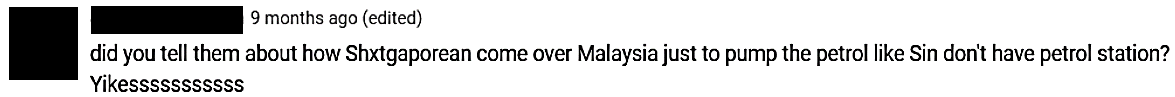
\includegraphics[width=\linewidth]{imagens/exemplo11.png}
    \caption{Example 11.}\label{example-11}
    \source{\cite{jocelyn2023malaysian}.}
    \end{minipage}
\end{figure}

Resonance can be found in Example 11 (\Cref{example-11}) when the user creatively replaced the first syllable ‘Sing’ of the word ‘Singaporean’ with a phonetically similar syllable ‘Shxt’. Similar to Examples \ref{example-9} and \ref{example-10}, this is a phonetic resonance as it involves a repetition of sounds \cite{tantucci2022a}. Furthermore, ‘Shxt’ is also a disguise of the intended swear word ‘shit’. Social media users sometimes disguise words to avoid YouTube detecting inappropriate or abusive language in the comment section, thus preventing their comments from being deleted.

\subsection{Resonance on joke lines: ``some jokes don’t land" and ``awwww boooo!!!"}
The social media users imitate Chia’s joke lines ``Some jokes don’t land" and ``Awwww boooo!!!" and alternate them into impoliteness to attack her in the comments.

%--- CÓDIGO DO EXEMPLO 12 ---%
\begin{figure}[h!]
    \centering
    \begin{minipage}{0.5\linewidth}
    
\includegraphics[width=\linewidth]{imagens/exemplo12.png}
    \caption{Example 12.}\label{example-12}
    \source{\cite{jocelyn2023malaysian}.}
    \end{minipage}
\end{figure}

The commenter in Example 12 (\Cref{example-12}) reuses the comedian’s original joke line by resonating it at multiple levels. At the syntactic level, the structure constructed by the comedian [NOUN AUX VERB] is resonated by the user through a mirrored structure [NOUN modifier AUX VERB]. At the pragmatic level, it overtly indicates a disagreement in which the illocutionary force of the user’s utterance is reinforced by resonating the original joke line of the comedian. This is observed when the user replaces and alters the auxiliary verb ``don’t" with ``really can" to indicate the contrary, which also shows a form of disagreement with the comedian (\Cref{tab-5}).

%--- CÓDIGO DA TABELA 5 ---%
\begin{table}[h!]
\centering
\begin{threeparttable}
\caption{Noun + aux + verb.}\label{tab-5}
\begin{tabular}{lllll}
\toprule
& Noun & Aux & Verb & Illocutionary force \\
\midrule
Original line & \emph{Some jokes} & don’t & \emph{land} & To state \\
Resonance & It & really can & \emph{land} & To disagree \\
\bottomrule
\end{tabular}
\source{Own elaboration.}
\end{threeparttable}
\end{table}

%--- CÓDIGO DO EXEMPLO 13 ---%
\begin{figure}[h!]
    \centering
    \begin{minipage}{0.80\linewidth}
    
\includegraphics[width=\linewidth]{imagens/exemplo13.png}
    \caption{Example 13.}\label{example-13}
    \source{\cite{jocelyn2023malaysian}.}
    \end{minipage}
\end{figure}


The user begins with an insult by calling the comedian \textit{‘aunty kiasu’} (aunty fear of missing out) in Example 13 (\Cref{example-13}), which is a common word in Singaporean English to indicate one is being overcompetitive, and \textit{‘anak dara tua’} (old virgin), to indicate she is unmarried despite being in her 40s. Resonance can be observed where the syntactic structure of the comedian’s utterance [Noun Aux Verb] echoed the user’s utterance [Noun Aux Verb]. The only feature that is replaced is the noun phrase (from ‘Some jokes’ to ‘Your funny’). Pragmatically, the illocutionary force of the comedian’s utterance is to state; whereas the user’s utterance is to insult the comedian when he changes the unspecified pronoun ‘some’ to the possessive pronoun ‘your’, directly insulting her with personalised negative reference (\Cref{tab-6}). 

%--- CÓDIGO DA TABELA 6 ---%
\begin{table}[h!]
\centering
\begin{threeparttable}
\caption{Noun + aux + verb.}\label{tab-6}
\begin{tabular}{lllll}
\toprule
& Noun & Aux & Verb & Illocutionary force \\
\midrule
Original line & \emph{Some jokes} & \emph{don’t} & \emph{land} & To state \\
Resonance & Your funny & \emph{don’t} & \emph{land} & To insult \\
\bottomrule
\end{tabular}
\source{Own elaboration.}
\end{threeparttable}
\end{table}

%--- CÓDIGO DO EXEMPLO 14 ---%
\begin{figure}[h!]
    \centering
    \begin{minipage}{0.5\linewidth}
    
\includegraphics[width=\linewidth]{imagens/exemplo14.png}
    \caption{Example 14.}\label{example-14}
    \source{\cite{jocelyn2023malaysian}.}
    \end{minipage}
\end{figure}


The user’s resonance in Example 14 (\Cref{example-14}) is constructed on a parallelism with Chia’s original joke line ``Some jokes don’t land" in the first half of the comment, despite having some grammatical errors. Nevertheless, he creatively constructs impoliteness towards Chia with the further addition of a direct insult: ``but your brain [sic] under my feet". From a pragmatic perspective, the illocutionary force of the original line is to inform that jokes are subjective as not everyone may find the same joke funny. However, similar to Example 13 (\Cref{example-13}), the illocutionary force of the resonance in Example 14 (\Cref{example-14}) is to insult the comedian for not considering the feelings of others when making jokes about Malaysia and the MH370 tragedy. It also portrays the commenter’s annoyance with the comedian (\Cref{tab-7}).

%--- CÓDIGO DA TABELA 7 ---%
\begin{table}[h!]
\centering
\begin{threeparttable}
\caption{Utterance + direct insult.}\label{tab-7}
\begin{tabular}{p{2cm} p{3.5cm} p{4cm} p{3cm}}
\toprule
& Utterance & Direct insult & Illocutionary force \\
\midrule
Original line & \emph{Some jokes don’t land} & -- & To state \\
Resonance & \emph{Some joke} [sic] \emph{don’t lane} [sic] & But your brain [sic] under my feet & To insult \\
\bottomrule
\end{tabular}
\source{Own elaboration.}
\end{threeparttable}
\end{table}

%--- CÓDIGO DO EXEMPLO 15 ---%
\begin{figure}[h!]
    \centering
    \begin{minipage}{0.5\linewidth}
    
\includegraphics[width=\linewidth]{imagens/exemplo15.png}
    \caption{Example 15.}\label{example-15}
    \source{\cite{jocelyn2023malaysian}.}
    \end{minipage}
\end{figure}


In Example 15 (\Cref{example-15}), the user draws on Chia’s original joke line ``Awwww booooo!! Fuck you, Malaysia" as a resource for producing new impolite expressions by reusing the first part of the utterance ``Awwww booooo!!" and replacing the latter ones with new utterances ``Your career will be end [sic] soon", which serves as a threat (\Cref{tab-8}).

%--- CÓDIGO DA TABELA 8 ---%
\begin{table}[h!]
\centering
\begin{threeparttable}
\caption{Interjection + direct insult.}\label{tab-8}
\begin{tabular}{lllll}
\toprule
& Interjection & Direct insult & Illocutionary force \\
\midrule
Original line & \emph{Awwww booooo!!} & Fuck you, Malaysia! & To joke \\
Resonance & \emph{Awwww booooo!!} & Your career will be end [sic] soon!! & To threaten \\
\bottomrule
\end{tabular}
\source{Own elaboration.}
\end{threeparttable}
\end{table}

%--- CÓDIGO DO EXEMPLO 16 ---%
\begin{figure}[h!]
    \centering
    \begin{minipage}{0.70\linewidth}
    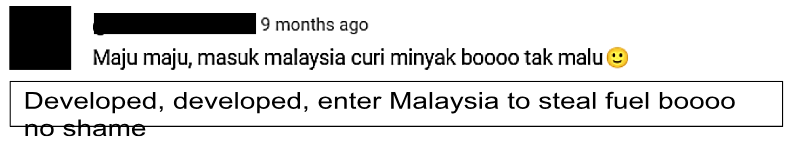
\includegraphics[width=\linewidth]{imagens/exemplo16.png}
    \caption{Example 16.}\label{example-16}
    \source{\cite{jocelyn2023malaysian}.}
    \end{minipage}
\end{figure}

%--- CÓDIGO DA TABELA 9 ---%
\begin{table}[h!]
\centering
\begin{threeparttable}
\caption{Interjection + direct insult.}\label{tab-9}
\begin{tabular}{lllll}
\toprule
& Interjection & Direct insult & Illocutionary force \\
\midrule
Original line & Awwww \emph{booooo!!} & Fuck you, Malaysia! & To joke \\
Resonance & \emph{Boooo} & \textit{tak malu} (no shame) & To condescend \\
\bottomrule
\end{tabular}
\source{Own elaboration.}
\end{threeparttable}
\end{table}

Unlike Example 15 (\Cref{example-15}), the user in Example 16 (\Cref{example-16}) begins with a condescension, \textit{``Maju maju, masuk malaysia curi minyak"} (``Developed, developed, enter Malaysia to steal fuel"), indicating that Singaporeans, who are from a developed country, have to come over to Malaysia to steal fuel. The condescension is then followed by the resonance construction [interjection + direct insult] \textit{``boooo tak malu"} (``boooo no shame"), which is a creative alteration of Chia’s original joke line (\Cref{tab-9}).

\section{Discussion}
This study reveals that insults were the most prominent conventionalised impoliteness trigger, while non-conventionalised triggers included sarcasms (external convention-driven implicational impoliteness) and mimicry or resonance (form-driven implicational impoliteness). These triggers were mainly employed to attack the comedian’s intellect for allegedly disregarding the consequences of her performance. Some users also extended their attacks to Chia’s personal matters, such as her name, nationality, age, marital status, and appearance.

A distinct feature of the responses in the findings was the creative use of resonance, where the YouTube users re-used Chia’s original words and constructed them in impolite ways, which is what \textcite{dubois2014} and \textcite{tantucci2021} term ‘dynamic’ or ‘creative resonance’. This appeared at multiple levels. On the word level, users creatively constructed impolite resonance to insult her name and Singaporean nationality. Phrase level can be observed when users alternated her original phrase line ``Some jokes" and turned it into direct attacks like ``Your funny [sic]". Sentence and/or utterance levels can be seen when users added insults such as ``Your brain [sic] under my feet" or ``Your career will be over [sic] soon!!" to juxtapose with Chia’s original joke lines ``Awww booo" and ``Some jokes don’t land". Additionally, we observed patterns of phonetic resonance where users disguised spellings of the intended swear words, such as ‘shxt’ (i.e., ‘shit’), ‘bij’ (i.e., ‘bitch’), and ‘Goblyn’ (i.e., ‘goblin’). The deliberate misspelling of words serves as an ``indirect addressivity tool" \cite[p. 153]{vladimirou2018}, allowing users to insult and mock the comedian while evading detection or content removal by YouTube.

This resonant mockery functioned as both participation in PIR and PER. Users perceived Chia’s controversial routine as impolite and responded accordingly, attempting to restore a perceived moral or social equilibrium. However, a notable mismatch emerged. While the audience extensively engaged in resonance and retaliation, the comedian herself did not engage in further public interaction or retaliation. Instead, she appeared to embrace the controversy as a means of publicity. As reported by a Singaporean newspaper -- The Straits Times \cite{soh2025} --, Chia expressed gratitude for the backlash surrounding her MH370 joke, stating that the fallout had, in fact, boosted her international comedy career. This response forms a mismatch between the audience’s retaliatory efforts and the comedian’s own strategic reframing of the incident. 

In terms of PER, the users who are driven by national affiliation or ideological alignment formed a temporary online community with shared epistemic and moral stances. For them, Chia represented an outsider who lacks the moral proximity to comment on MH370. Their use of impoliteness strategies and resonance can be interpreted as a form of epistemic retaliation and also as a way to assert epistemic rights and community boundaries. This highlights how digital communication can lead to dynamic negotiations of social and epistemic authority. 

\section{Conclusion}
Traditionally, public figures like comedians hold top-down epistemic authority, where they perform while audiences passively listen. However, the rise of social media has redistributed this power horizontally, allowing audiences or viewers to co-construct meaning and judgment through public commentary and collective ridicule. In the case of Jocelyn Chia, her performative authority on stage, specifically her joke referencing Malaysia-Singapore relations and the MH370 tragedy, was contested by online users who drew on national identity, shared ideology, and collective memory to reject her epistemic stance and reassert their own. Although Chia claimed she meant no offense and was merely fulfilling her role as a stand-up comedian, audiences perceived her performance as epistemically inappropriate due to her lack of emotional proximity to these sensitive issues. This perceived mismatch triggered responses marked by impoliteness, resonance, and creative mockery, strategies that reflect ludic impoliteness, where mockery serves both to challenge Chia’s face and to entertain others. Importantly, as social media users were under no obligation to respond, their voluntary participation further emphasized their reclaimed epistemic authority in this public contestation.

This study offers theoretical novelty in impoliteness research by showing how resonance functions not only as a stylistic tool for creative impoliteness, but also as a strategic means of intensifying face attacks in social media discourse. Through shared language patterns, repeated phrasing, and intertextual mimicry, users creatively manipulate impoliteness not merely to insult, but to signal alignment, reinforce shared values, and build solidarity with like-minded others. This provides an insightful lens for pragmatic researchers to examine how hostile language is replicated, modified, and spread rapidly in multilingual online settings. The study offers a more localized understanding of impoliteness and resonance in an Asian context, particularly Malaysian. These findings imply that theories of impoliteness must account for the dynamic, creative, and multilingual ways hostile language spreads online. Thus, the study advances both methodologically and theoretically by bridging online multilingual data with core concepts in impoliteness research. 

Additionally, social media platforms like YouTube are not only spaces for entertainment but are also increasingly used as learning environments \cite{desouza2025, oliveira2023}. This dual function highlights the importance of critically understanding the type of language exposure that shapes users’ communicative norms.

One key limitation of this study is the absence of detailed demographic information about the commenters. While a few users explicitly mentioned their nationality (i.e., Malaysians), the majority did not, and no assumptions were made. Due to the user anonymity and ethical considerations regarding confidentiality, personal details were deliberately excluded from the analysis. As a result, interpretations were made without specific reference to individual demographic variables, which may influence language use and perception. 

Future research could address this by exploring more controlled or identifiable datasets to further contextualize these findings. Additionally, this study could be expanded by exploring the use of resonance in impoliteness across different languages or by conducting comparative analyses of its usage in two or more linguistic contexts.


\printbibliography\label{sec-bib}
% if the text is not in Portuguese, it might be necessary to use the code below instead to print the correct ABNT abbreviations [s.n.], [s.l.]
%\begin{portuguese}
%\printbibliography[title={Bibliography}]
%\end{portuguese}


%full list: conceptualization,datacuration,formalanalysis,funding,investigation,methodology,projadm,resources,software,supervision,validation,visualization,writing,review
\begin{contributors}[sec-contributors]
\authorcontribution{Cherish How}[conceptualization,investigation,formalanalysis,methodology,projadm,supervision,validation,writing,review]
\authorcontribution{Najah Zainal Abidin}[formalanalysis,investigation,writing,review]
\authorcontribution{Nur Azwin Zulkarnain}[investigation,formalanalysis,writing,review]
\end{contributors}



\end{document}

